\documentclass{article}

\usepackage{natbib}
\usepackage[utf8]{inputenc}
\usepackage[english]{babel}
\usepackage{natbib}
\usepackage{hyperref}
\usepackage{adjustbox}
\usepackage{eurosym}
\bibliographystyle{apalike}

\title{Ecological performance of detecting data fabrication with summary statistics}
\author{Chris HJ Hartgerink, Jan G Voelkel, Jelte M Wicherts, Marcel ALM van Assen\\
Preregistration conducted by first author}

\usepackage{Sweave}
\begin{document}
\input{manuscript-concordance}
\maketitle

Any field of empirical inquiry is faced with cases of scientific misconduct at some point, either in the form of fabrication, falsification or plagiarism (FFP). 
% Psychology was faced with Stapel; medical sciences were faced with Poldermans and Macchiarini; life sciences were faced with Voignet. These are just a few examples of cases in the last decade. Overall, an estimated 2\% of all scholars have admitted to falsifying or fabricating research results at least once \citep{fanelli2009} and this is likely to be an underestimate due to socially desirable responses. The detection rate is likely to be even lower; for example, only around a dozen cases are discovered in the United States and the Netherlands, despite covering several hundreds of thousands of researchers. At best, this amounts to a detection rate far below 1\% of those 2\% who admit to fabricating data --- the tip of a seemingly much larger iceberg.

In order to stifle attempts at data fabrication, improved detection of fabricated data is considered to deter such harmful attempts. 
% Although deterrence theory dates back to the middle of the 17th century \citep{leviathan}, its implementation has not occurred across the different forms of scientific misconduct equilaterally. Basically, deterrence theory stipulates that with increased risk of detection, the utility of scientific misconduct (for this context) will decrease and therefore fewer people will engage in such behaviors. This principle of deterrence has been implemented with plagiarism scanners, a development that already started a long time ago  \citep[e.g.,][]{Parker89computeralgorithms}. However, increased deterrence of fabrication and falsification by improved detection mechanisms has not been as widely implemented. 

In the last decade, detecting image manipulation has become one of the few forms of detecting scientific misconduct other than plagiarism.
% The Journal of Cell Biology scans each submitted image for potential manipulation \citep{The_Journal_of_Cell_Biology2015-vh}, which greatly increases the risk of detecting (blatant) image manipulation. More recently, algorithms have been developed to automate the scanning of images for (subtle) manipulations \citep{Koppers2016}. These developments in detecting image manipulation have increased detection risk during the pre-publication and post-publication phase by improving detection mechanisms and increasing the understanding of how images might be manipulated. Moreover, their application also helps researchers systematically evaluate research articles to estimate the extent of the problem of image manipulation \citep[4\% of all papers are estimated to contain manipulated images;][]{Bik06072016}. 

Statistical methods can provide one way to improve detection of data fabrication in empirical research. Humans are notoriously bad at understanding and estimating probabilities \citep[e.g.,][]{tversky1974, Tversky1971}, which could manifest itself in the fundamentally probabilistic data they try to fabricate. 
% That researchers do not understand probabilistic processes also presents itself in the interpretation of genuine research data \citep{Hoekstra2006, Sijtsma2015-ts, Goodman_1999}. When data are fabricated, probabilistic principles are easily violated if these principles are forgotten at the univariate level, bivariate level, trivatiate level, or beyond \citep{Haldane1948-nm}. Based on such a theoretical framework, statistical methods that investigate whether the reported data are actually plausible under theoretically probabilistic processes can be used to detect potential data fabrication. 

The application of such statistical methods to detect data fabrication has occurred in several cases in recent years and has potential for future application beyond a case-basis. 
% For example, problems with papers by Fuji were highlighted with statistical methods \citep{Carlisle2012-yg,Carlisle2015-wm}, resulting in 183 retractions \citep{oransky2015}. In this case, baseline measures across randomized groups were examined for too little variation. Random assignment should introduce a certain degree of random error that is might be missed by a human fabricator, misestimating the probabilistic process that generates such error. Another two cases are those of Sanna and Smeesters, where fabricated data were also detected with statistics \citep{simonsohn2013}. These cases inspected the variance of variances (i.e., the second level, or meta, variance). Once again, too little variation was what revealed problems in these data. These methods, although developed in a case-setting, need not be limited to cases. The application of such methods can be (semi-)automated if data are available in a machine-readable format that one of the statistical methods can be applied to. An example of such a potential case for mass application of using statistics to detect (potential) data fabrication is in the ClinicalTrials.gov database, where baseline measures across randomized groups are readily available for download and subsequent analysis \citep{Hartgerink2015-bm}.

Nonetheless, considering the potential harm of applying statistical methods to flag potentially problematic results, it needs to be sorted out whether such methods have diagnosticity that actually makes it responsible to apply them. 
% We hardly know how researchers might go about fabricating data. Cases such as Fuji, Smeesters, and Sanna provide some insights, but are highly pre-selected (i.e., those who got caught/confessed) and as such, systematically biased. Relatively extensive descriptions in rare and partial autobiogrophical accounts provide little insight into the actual data fabrication process, except for the setting where it might take place \citep[e.g., late at night when no one is around;][]{stapel_book}. Additionally, the performance of methods to detect data fabrication is highly dependent on the unknown  prevalence of data fabrication and the power to actually to detect data fabrication. Given that we do not know how researchers might fabricate data, the diagnosticity of these methods cannot realistically be simulated.

The effectiveness of detection mechanisms and their consequences, hence their expected deterrence, is exacerbated by the increased usage of public online discussion platforms such as PubPeer (\url{https://pubpeer.com}). 
% PubPeer serves as an "online journal club" where anyone can discuss articles. Authors are notified when someone leaves a response, providing them with the possibility to respond. Such a platform allows for public discussion of the paper, including discussion of reanalyses, methodology, availability of materials, etc. When detection mechanisms are freely available to use, they can lead to (a surge of) comments when applied by users. Recently, in 2016, one user (the main author of this paper) used `statcheck` software to report potential statistical reporting inconsistencies for 50,000 psychology articles, which led to a large discussion about (automated) online comments \citep{Baker_2016}. The impact of such new possibilities is not to be underestimated, although its potential to contribute to the scientific discussion should also not be. Nonetheless, the `statcheck` software was well validated prior to this application \citep{Nuijten_2015} and the same principle applies to the application of statistical methods to detect (potential) data fabrication.

Throughout this paper, we inspect statistical methods to detect data fabrication that can be applied to (1) summary results or (2) raw data. 
% Even though the data available can look different depending on the structure of a study, there are certain common characteristics of results and the underlying raw data that can be inspected. For example, summary results frequently include means, standard deviations, test-statistics, and $p$-values. Raw data frequently contain at least some variables measured at a interval- or ratio scale \citep{Stevens_1946}.

We present a set of studies that directly test the validity of statistical methods to detect data fabrication. 
% To this end, Study 1 inspected the performance of statistical methods to detect data fabrication when using only summary results (e.g., means and standard deviations) as typically reported in empirical research articles. Study 2 inspected the performance of statistical methods aimed at detecting data fabrication in raw data (i.e., the data underlying summary results). These two studies provide a first indication of how applicable and effective statistical methods are to detect data fabrication in practice, with actual researchers fabricating actual data.


\section*{Study 1}


We tested the performance of statistical methods to detect data fabrication in summary results with genuine- and fabricated summary results from four anchoring studies \citep{tversky1974,jacowitz1995}. The anchoring effect is a well-known psychological heuristic that uses the information in the question as the starting point for the answer, which is then adjusted to yield a final estimate of a quantity. For example 'Is the percentage of African countries in the United Nations more or less than [10\% or 65\%]?'. These questions yield mean responses of 25\% and 45\%, respectively \citep{tversky1974}, despite essentially posing the same factual question. A considerable amount of genuine datasets on this heuristic are freely available and we collected fabricated datasets within this study. All described methods were approved by the Tilburg Ethical Review Board (EC-2015.50).

\subsection*{Methods}

We collected summary results for four anchoring studies: (i) distance from San Francisco to New York, (ii) population of Chicago, (iii) height of the Mount Everest, and (iv) the number of babies born per day in the United States \citep{jacowitz1995}. Each of the four studies provided us with summary results for a 2 (low/high anchoring) $\times$ 2 (male/female) factorial design. Throughout this study, the unit of analysis is a set of summary statistics (i.e., means, standard deviations, and test results) for the four anchoring studies from one respondent. For current purposes, a respondent is defined as researcher/lab where the four anchoring studies' summary statistics originate from. All materials, data, and analyses scripts are freely available on the OSF (\url{https://osf.io/b24pq}) and a preregistration is available at \url{https://osf.io/ejf5x} (deviations are explicated in this report).

\subsubsection*{Data collection}

We downloaded thirty-six genuine datasets from the publicly available Many Labs (ML) project \citep[\url{https://osf.io/pqf9r};][]{klein2014}. The ML project replicated several effects across thirty-six locations, including the anchoring effect in the four studies mentioned previously. Considering the size of the ML project, the transparency of research results, and minimal individual gain for fabricating data, we assumed these data to be genuine. For each of the thirty-six locations we computed sample sizes, means, and standard deviations for each of the four conditions in the four anchoring studies (i.e., $3\times4\times4$) for each of the thirty-six locations. We computed these summary statistics from the raw ML data, which were cleaned using the original analysis scripts from the ML project.

Using quotum sampling, we collected thirty-six fabricated datasets of summary results for the same four anchoring studies. Quotum sampling was used to sample as many responses as possible for the available 36 rewards (i.e., not all respondents might request the gift card and count towards the quotum; one participant did not request a reward). The sampling frame consisted of 2,038 psychology researchers who published a peer-reviewed paper in 2015, as indexed in Web of Science (WoS) with the filter set to the U.S. We sampled psychology researchers to improve familiarity with the anchoring effect \citep{jacowitz1995,tversky1974}, for which summary results were fabricated. We filtered for U.S. researchers to ensure familiarity with the imperial measurement system, which is the scale of some of the anchoring studies (note: we found out several non-U.S. researchers were included because the WoS filter also retained papers with co-authors from the U.S.). WoS was searched on October 13, 2015. In total, 2,038 unique corresponding e-mails were extracted from 2,014 papers (due to multiple corresponding authors).

We invited a random sample of 1,000 researchers via e-mail to participate in this study on April 25, 2016 (invitation: \url{https://osf.io/s4w8r}). The study took place via Qualtrics with anonimization procedures in place (e.g., no IP-addresses saved). We informed the participating researchers that the study would require them to fabricate data and explicitly mentioned that we would investigate these data with statistical methods to detect data fabrication. We also clarified to the  respondents that they could stop at any time without providing a reason. If they wanted, respondents received a \$30 Amazon gift card as compensation for their participation if they were willing to enter their email address. They could win an additional \$50 Amazon gift card if they were one of three top fabricators. The provided e-mail addresses were unlinked from individual responses upon sending the bonus gift cards. The full text of the Qualtrics survey is available at \url{https://osf.io/w984b}.

Each respondent was instructed to fabricate 32 summary statistics (4 studies $\times$ 2 conditions $\times$ 2 sexes $\times$ 2 statistics [mean and sd]) that fulfilled three hypotheses. We instructed respondents to fabricate results for the following hypotheses: there is (i) a main effect of condition, (ii) no effect of sex, and (iii) no interaction effect between condition and sex. We fixed the sample sizes to 25 per cell; respondents did not need to fabricate sample sizes. The fabricated summary statistics and their accompanying test results for these three hypotheses serve as the data to examine the properties of statistical tools to detect data fabrication.

We provided respondents with a template spreadsheet to fill out the fabricated data, in order to standardize the fabrication process without restraining the participant in how they chose to fabricate data. Figure \ref{fig1} depicts an example of this spreadsheet (original:  \url{https://osf.io/w6v4u}). We requested respondents to fill in the yellow cells with fabricated data, which includes means and the standard deviations for four conditions. Using these values, statistical tests are computed and shown in the "Current result" column instantaneously. If these results confirmed the hypotheses, a checkmark appeared as depicted in Figure \ref{fig1}. We required respondents to copy-paste the yellow cells into Qualtrics, to provide a standardized response format that could be automatically processed in the analyses.

\begin{figure}
\begin{center}
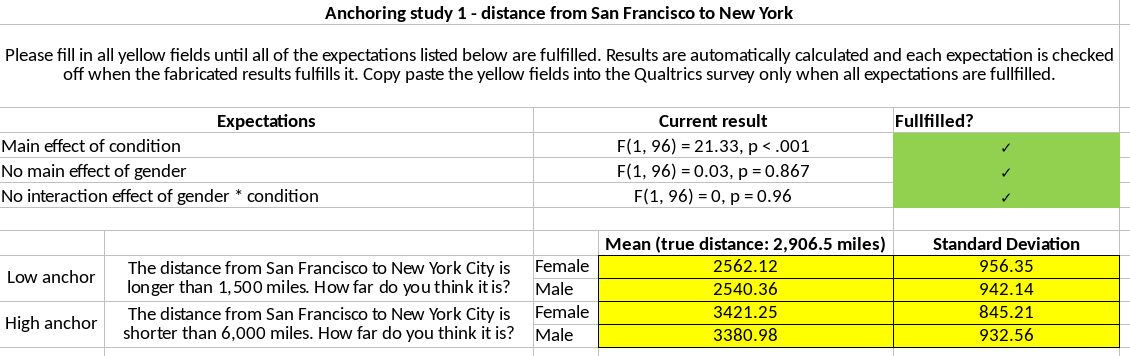
\includegraphics[width=\textwidth,height=\textheight,keepaspectratio]{../figures/spreadsheet.png}
\caption{Example of a filled in template spreadsheet used in the fabrication process of Study 1. Respondents fabricated data in the yellow cells, which were used to compute the results of the hypothesis tests. If the fabricated data confirm the hypotheses, a checkmark appeared in a green cell (one of four template spreadsheets available at \url{https://osf.io/w6v4u/}).}
\label{fig1}
\end{center}
\end{figure}

Upon completing the fabrication of the data, respondents were debriefed. Respondents answered several questions about their statistical knowledge and approach to data fabrication and finally we reminded them that data fabrication is widely condemned by professional organizations, institutions, and funding agencies alike. We rewarded participation with a \$30 Amazon gift card and the fabricated results that were most difficult to detect received a bonus \$50 Amazon gift card.

\subsubsection*{Data analysis}

To detect data fabrication in a set of summary results, we first tested the standardized standard deviations (SDs) for data fabrication \citep{simonsohn2013} across the four anchoring studies. This method tests whether the observed SDs contain a reasonable amount of variation, as expected based on random sampling processes. For example, if four independent samples all yield the variance $2.22$, this could be considered excessively consistent when the probability that this amount of consistency (or more) is less than 1 out of 1000 in truly random samples. To compute this probability, we first standardized the SDs for each of the four studies with
\begin{equation}
z_j=\sqrt{\frac{s^2_j}{MS_w}}=\sqrt{\frac{s^2_j}{\left(\frac{\sum\limits^k_{j=1}(N_j-1)s^2_j}{\sum\limits^k_{j=1}(N_j-1)}\right)}}
\label{s2_j}
\end{equation}
where $z_j$ denotes the standardized SD in group $j$ ($MS_w$ is the simple arithmetic mean when sample sizes are equal for all cells, which is the case for the fabricated datasets). We tested different measures to detect data fabrication that utilize these standardized SDs (i.e., $z_j$). We included the variance of the standardized SDs \citep[i.e.,  $SD_{z}$;][]{simonsohn2013} and tried out the max-min distance of the standardized SDs (denoted $max-min_{z}$) as an alternative measure. We compared the observed value for each measure with the expected distribution when the summary results are used to generate random samples. To this end, we simulated the expected distribution of standardized SDs and computed the expected distribution of each measure. This expected distribution was used to determine the $p$-value of the observed $SD_z$ and $max-min_z$. We simulated the standardized variance for each of the $j$ groups as
\begin{equation}
z^2_j\sim\left(\frac{\chi^2_{N_j-1}}{N_j-1}\right)/MS_w
\label{simvar}
\end{equation}
These simulated values are used to compute the expected distribution of the $SD_z$ and $max-min_z$  measures.

Testing the standardized SDs for potential data fabrication can be done either for each study separately or all studies combined; the test can also be done under different assumptions of population variances across conditions. The assumptions of population variance can either by that all SDs originate from the same distribution \citep[as in][]{simonsohn2013}, the SDs within a factor are from the same distribution, or each group comes from its own distribution. We preregistered the method that assumes the SDs are drawn from the same distribution for the various conditions (i.e., homogeneous SDs) and are tested across all studies. However, upon conducting the analyses, we decided homogenous SDs are not unequivocal and included computations where the SDs for the low anchor and high anchor are from different distributions (i.e., heterogeneous SDs). Additionally, the signal for data fabrication across the four anchoring studies might result in different studies cancelling each other out, so we also included analyses where each study was analyzed separately.

Second, we applied the reversed Fisher method to detect data fabrication to the nonsignificant $p$-values twice: once for the results of gender effects hypothesis in each study and once for the results of the interaction effect hypothesis for each study. The Fisher method \citep{fisher1925} tests for evidence of an effect in a set of $p$-values by testing for a right-skew $p$-value distribution, but we adjusted it here to test for results that are overly consistent with the null hypothesis and result in a left-skew distribution (see Figure \ref{leftskew}). The original Fisher method is computed as
\begin{equation}
\chi^2_{2k}=-2\sum\limits^k_{i=1}\ln(p_i)
\label{fishertest}
\end{equation}
and tests for right-skew in a set of $p$-values, but we adjust it to the following
\begin{equation}
\chi^2_{2k}=-2\sum\limits^k_{i=1}\ln(1-\frac{p_i-t}{1-t})
\label{fisheradjusted}
\end{equation}
where it now tests for left-skew (i.e., more larger $p$-values than smaller $p$-values) across the $k$ number of $p$-values that falls above the threshold $t$. We set this threshold to .05 in order to include only nonsignificant test results. The theoretical idea behind this method is that researchers who fabricate nonsignificant data might forget to fabricate a uniform $p$-value distribution, given the frequent misinterpretation of $p$-values \citep[e.g., as the probability of an effect,][]{Goodman2008135,Altman_1995}. % I can add more refs but it is just a rabbit hole to start with more.


% add plot of left and right skew
\begin{figure}[!ht]
\begin{center}
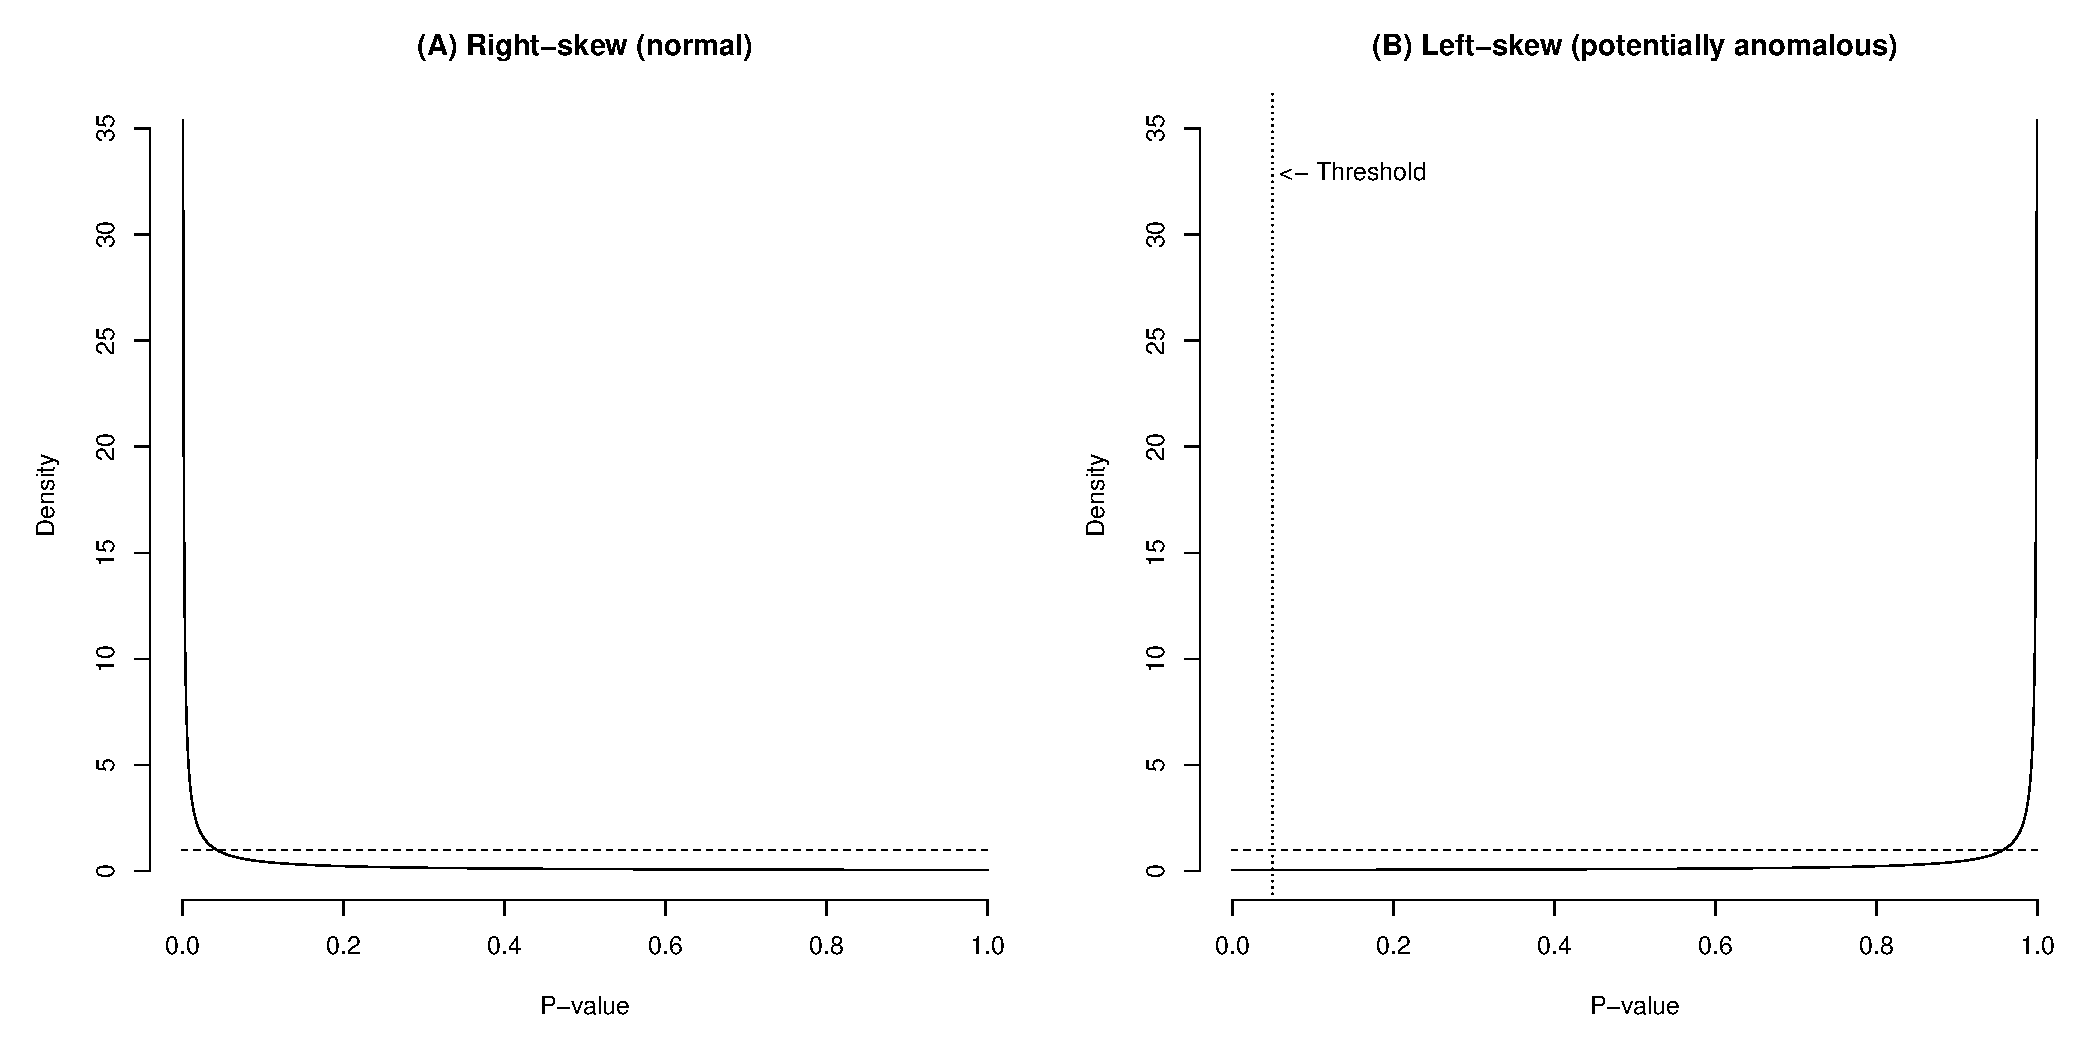
\includegraphics[width=\textwidth,height=\textheight,keepaspectratio]{../figures/fisherfig.pdf}
\caption{Conceptual representation of what the Fisher test inspects (Equation \ref{fishertest}; panel A) and what the adjusted Fisher test inspects (Equation \ref{fisheradjusted}; panel B). Both panels test whether there is sufficient evidence that the solid line deviates from the dashed line, except that the type of deviation that the test is sensitive to is the exact opposite.}
\label{leftskew}
\end{center}
\end{figure}

Finally, we combined the aforementioned methods to detect data fabrication with the Fisher method. This included the $SD_z$ measure across all studies and the Fisher test (Equation \ref{fisheradjusted}) of the gender hypothesis test and the interaction test.  We expected this combination test of the three individual tests for data fabrication to be more powerful than the individual tests, given that these tests inspect different manifestations of data fabrications. Based on the results of the combined test results, the three least detectable data fabricators were selected. The three respondents with the highest $p$-values on this combined method to detect data fabrication contained the least evidential value for deviating from genuine data and received an additional \$50 Amazon gift card.

For each of these four tests to detect data fabrication ($SD_z$, Fisher test for the gender and interaction hypotheses, combined methods) we carried out sensitivity and specificity analyses using ROC-curves. ROC-analyses indicate the sensitivity (i.e., True Positive Rate [TPR]) and specificity (i.e., True Negative Rate [TNR]) for various decision criteria (e.g., $\alpha=0, .01, .02, ..., .99, 1$). With these ROC-curves, informed decisions about optimal alpha levels can be made based on various criteria. In this case, we determine the optimal alpha level by finding that alpha level for which the combination of TPR and TNR were highest. For example, if $\alpha=.04$ results in $TPR=.30$ and $TNR=.70$, but $\alpha=.05$ results in $TPR=.5$ and $TNR=.5$, .05 was chosen as an optimal decision criterion based on the sample. 
% Maybe include bootstrapped errors here.

\subsection*{Results}


The collected data included 36 genuine data from Many Labs 1 \citep[\url{https://osf.io/pqf9r};][]{klein2014} and 39 fabricated datasets(\url{https://osf.io/e6zys}; 3 participants did not participate for a bonus). 

Figure \ref{densities} shows a group-level comparison of the genuine- and fabricated $p$-values and effect sizes ($r$). Such group-level comparisons provide an overview of the differences between the genuine- and fabricated data \citep[see also][]{Akhtar-Danesh2003}. These distributions indicate little group differences between genuine- and fabricated data when nonsignificant effects are inspected (i.e., gender and interaction hypotheses) whereas there seem to be large group differences when we required subjects to fabricate significant data (i.e., condition hypothesis). From our own experience, and anecdotal evidence elsewhere \citep{BAILEY1991741}, large effects have previously raised initial suspicions. These data corroborate the idea that extremely large effect sizes (e.g., $r>.95$) might prove to be an easy-to-implement flag for potentially anomalous data (it is wise to seek for alternative explanations after flagging, however). Considering this, we also investigated how well effect sizes perform in detecting data fabrication (not preregistered). In the following sections, we investigate the performance of such statistical methods to detect data fabrication on an respondent-level basis.

% add plot of left and right skew
\begin{figure}[!ht]
\begin{center}
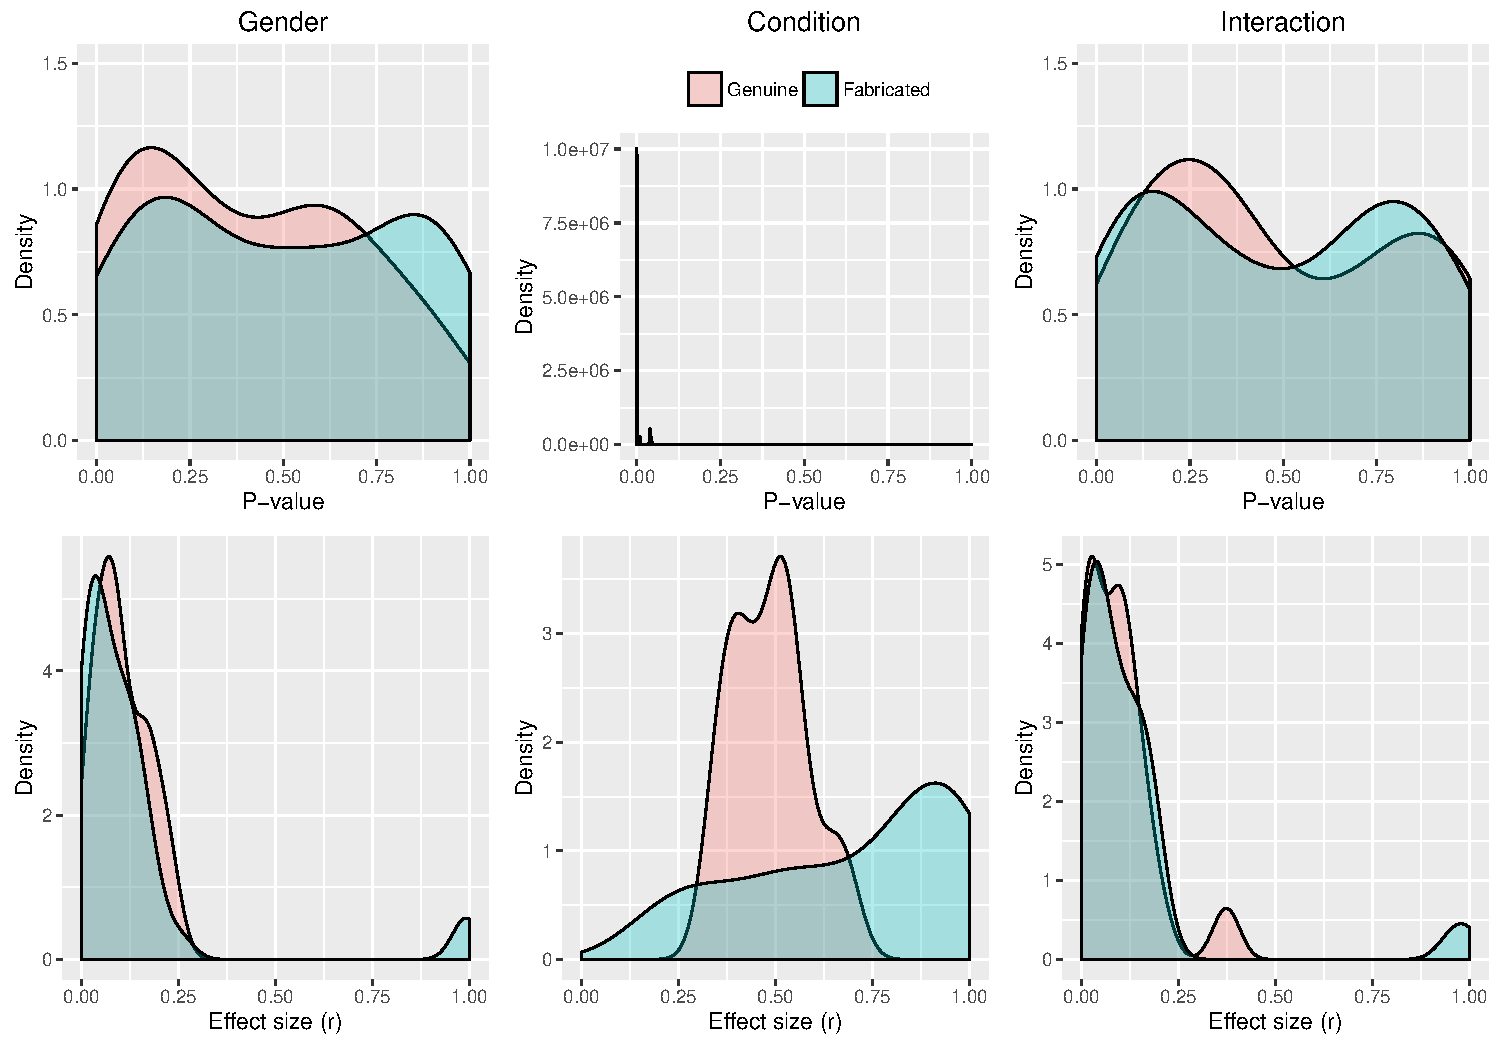
\includegraphics[width=\textwidth,height=\textheight,keepaspectratio]{../figures/ddfab_density.pdf}
\caption{Overlay of density distributions for both genuine and fabricated data, per effect and type of result. We instructed respondents to fabricate nonsignificant data for the gender and interaction effects, and a significant effect for the condition effect.}
\label{densities}
\end{center}
\end{figure}


\subsubsection*{Performance of using SDs to detect data fabrication}

We applied two different operationalizations to inspect for data fabrication in the genuine- and fabricated datasets based on variance in the SDs. The $SD_z$ method \citep{simonsohn2013} inspects whether the variance of the SDs themselves varies sufficiently, and we tested another method that inspects the range of the SDs varies sufficiently. These two methods operate similarly, except for the final computation. Other operationalizations are possible and we invite others to reuse the data from this study (\url{https://osf.io/b24pq}).

Table \ref{auroc_variances} indicates that both methods show similar performance when inspected with the Area Under the Receiver Operating Curve (AUROC), but with a preference for $SD_z$. This preference is due to the variance of variances outperforming the range of variances when all studies are combined in one test and its past application \citep{simonsohn2013}. Throughout the rest of this section, we will only discuss the results of $SD_z$ further.

% latex table generated in R 3.3.3 by xtable 1.7-1 package
% Tue Apr 18 19:23:42 2017
\begin{table}[ht]
\centering
\begin{tabular}{lrr}
  \hline
Method & AUROC $SD_z$ & AUROC $maxmin_z$ \\ 
  \hline
Homogeneous, all studies combined & 0.423 & 0.303 \\ 
  Homogeneous, study 1 & 0.368 & 0.374 \\ 
  Homogeneous, study 2 & 0.421 & 0.446 \\ 
  Homogeneous, study 3 & 0.510 & 0.521 \\ 
  Homogeneous, study 4 & 0.540 & 0.542 \\ 
  Heterogeneous, all studies combined & 0.770 & 0.756 \\ 
  Heterogeneous study 1, low anchor condition & 0.643 & 0.643 \\ 
  Heterogeneous study 1, high anchor condition & 0.438 & 0.438 \\ 
  Heterogeneous study 2, low anchor condition & 0.751 & 0.751 \\ 
  Heterogeneous study 2, high anchor condition & 0.612 & 0.612 \\ 
  Heterogeneous study 3, low anchor condition & 0.668 & 0.668 \\ 
  Heterogeneous study 3, high anchor condition & 0.651 & 0.651 \\ 
  Heterogeneous study 4, low anchor condition & 0.796 & 0.796 \\ 
  Heterogeneous study 4, high anchor condition & 0.555 & 0.555 \\ 
   \hline
\end{tabular}
\caption{Area Under the Receiver Operating Curve (AUROC) for the two statistical methods used to detect data fabrication based on variances. Homogeneous: assumes one population variance underlying all groups. Heterogeneous: assumes separate population variance per anchoring condition.} 
\label{auroc_variances}
\end{table}
The AUROC indicates the probability that a randomly drawn fabricated dataset is classified as fabricated before a randomly drawn genuine dataset is classified as fabricated \citep{doi:10.1148/radiology.143.1.7063747}. In other words, if AUROC $=.5$ this indicates that correctly classifying a randomly drawn dataset in this sample is equal to a coin flip. For this setting, we will regard any AUROC $<.6$ as plainly insufficient for detecting data fabrication, $.6\leq$ AUROC $<.7$ as failed, $.7\leq$ AUROC $<.8$ as sufficient, $.8\leq$ AUROC $<.9$ as good, and $.9\leq$ AUROC $\leq 1$ as excellent.

The AUROC for the variance of variance analyses is insufficient or sufficient depending on the assumption regarding population variances. Table \ref{auroc_variances} indicates that AUROC $=.423$ when homogeneous population variances are assumed, whereas AUROC $=.770$ when heterogeneous population variances are assumed. For the anchoring studies, homogeneous population variances across conditions seem unreasonable and greatly affect the performance of the statistical method. The method that incorporates heterogeneous population variances (i.e., one per anchoring condition) greatly improves the performance of the variance of variances analysis.

Further inspecting the heterogeneous variance of variances analysis indicates that no false positives occur until $\alpha=0.13$. 

\subsubsection*{Performance of using $p$-values to detect data fabrication}

We asked researchers to fabricate data for nonsignificant effect sizes after inspecting whether the genuine data resembled a uniform distribution. Consequently,  However, as Table \ref{auroc_fisher} indicates, the auroc for these methods are hardly better than chance. In other words, for effects that are specifically fabricated to be nonsignificant, researchers might not fabricate such large $p$-values to be suspicious.

% latex table generated in R 3.3.3 by xtable 1.7-1 package
% Tue Apr 18 19:23:42 2017
\begin{table}[ht]
\centering
\begin{tabular}{lr}
  \hline
Method & AUROC \\ 
  \hline
Fisher test gender hypothesis & 0.521 \\ 
  Fisher test interaction hypothesis & 0.535 \\ 
   \hline
\end{tabular}
\caption{Area Under the Receiver Operating Curve (AUROC) for PLACEHOLDER} 
\label{auroc_fisher}
\end{table}
\subsubsection*{Performance of combining SDs and $p$-value methods to detect data fabrication}

% latex table generated in R 3.3.3 by xtable 1.7-1 package
% Tue Apr 18 19:23:42 2017
\begin{table}[ht]
\centering
\begin{tabular}{lr}
  \hline
Method & AUROC \\ 
  \hline
Combined Fisher test (3 results, $SD_z$ homogeneous) & 0.602 \\ 
  Combined Fisher test (3 results, $SD_z$ heterogeneous) & 0.736 \\ 
  Combined Fisher test (6 results, $SD_z$ homogeneous) & 0.643 \\ 
  Combined Fisher test (6 results, $SD_z$ heterogeneous) & 0.643 \\ 
   \hline
\end{tabular}
\caption{Area Under the Receiver Operating Curve (AUROC) for PLACEHOLDER} 
\label{auroc_combined}
\end{table}

\subsubsection*{Performance of large effect sizes to detect data fabrication}


%The 23 largest significant effects were fabricated, with 13 (0.333\%) larger than $r=.9$. Based on descriptive data throughout psychology \citep{Hartgerink2016-lg}, effect sizes $\geq.9$ belong to the 96th percentile of effects throughout the psychology literature and effect sizes $\geq.95$ 98th percentile.


\subsection*{Discussion}

% variance analysis and effect size best ways to inspect
% but severely correlated: smaller variances = larger effects
% easiest way is too look for massive effects in the effects

% Simonsohn method not invalid under homogeneous, just somethign to take into account
% easily adjusted

% Discuss how the PPV is likely to be overestimated because prevalence is 50% in this study
% How we don't know the prevalence, in fact.

% Discuss alpha choice based on sample has large error (small sample).
% Only provides a first indication

% Comparison between methods not tested, large error given small sample.
% This provides just initial work


\section*{Study 2}

In Study 2 we investigated detecting data fabrication in raw data as an extension of Study 1, which presented results of detecting data fabrication in summary results. In essence, the procedure is similar: we asked actual researchers to fabricate data that they thought would go undetected. For Study 2 we included a face-to-face interview to qualitatively assess how data fabrication occurs. A preregistration of this study occurred during the seeking of funding \citep{10.3897/rio.2.e8860} and during data collection (\url{https://osf.io/XXXX}).

To test the validity of statistical methods to detect data fabrication in raw data, we investigated raw data of a Stroop experiment \citep{Stroop_1935}. In the Stroop task, participants are asked to determine the color a word is presented in (i.e., word colors), but the word also reads a color (i.e., color words). The presented word color (i.e., 'red', 'blue', or 'green') can be either presented in the congruent color (e.g., 'red' presented in red) or an incongruent color (i.e., 'red' presented in green). The dependent variable in the Stroop task is the response latency (in this study milliseconds are used). Participants in actual studies are typically presented with a set of these, where the mean and standard deviation per condition serves as the raw data. The Stroop effect typically is computed as the difference in mean response latencies between the congruent and incongruent conditions.

\section*{Methods}


Twenty-one genuine datasets on the Stroop task were collected from the Many Labs 3 project \citep[\url{https://osf.io/n8xa7/};][]{Ebersole201668}. Many Labs 3 (ML3) includes 20 participant pools from universities and one online sample \citep[the original preregistration mentioned 20 datasets, accidentally overlooking the online sample;][]{10.3897/rio.2.e8860}. Using the original raw data and analysis script from ML3 (\url{https://osf.io/qs8tp/}), we computed the mean (M) and standard deviation (SD) for the participant's response latencies in both the within-subjects conditions of congruent trials and incongruent trials. These also formed the basis for the template of the data that needed to be fabricated by the participants (see also Figure \ref{spreadsheet2}). The Stroop effect was calculated as a $t$-test of the difference ($H_0:\mu=0$).

\begin{figure}
\begin{center}
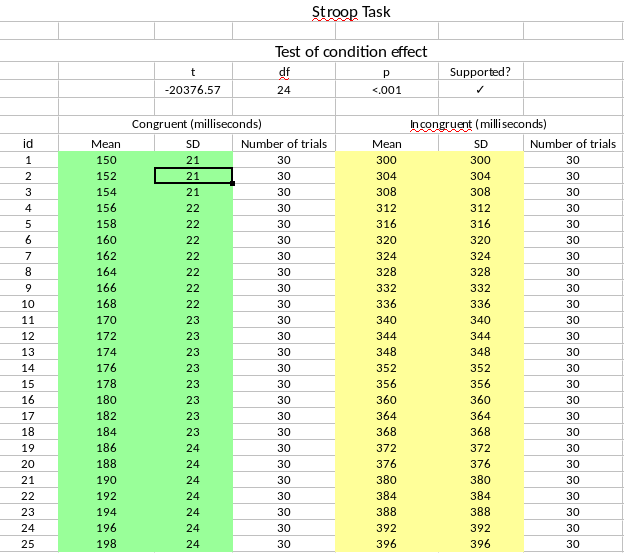
\includegraphics[width=\textwidth,height=\textheight,keepaspectratio]{../figures/spreadsheet2.png}
\caption{Example of a filled in template spreadsheet used in the fabrication process for Study 2. Respondents fabricated data in the yellow cells and green cells, which were used to compute the results of the hypothesis test of the condition effect. If the fabricated data confirm the hypotheses, a checkmark appeared. This template is available at \url{https://osf.io/2qrbs/}.}
\label{spreadsheet2}
\end{center}
\end{figure}

We collected twenty-eight faked datasets on the Stroop task experimentally in a two-stage sampling procedure. First, we invited 80 Dutch and Flemish psychology researchers who published a peer-reviewed paper on the Stroop task between 2005-2015 as available in the Thomson Reuters’ Web of Science database. We selected Dutch and Flemish researchers to allow for a face-to-face interview on how the data were fabricated. We chose the period 2005-2015 to prevent a drastic decrease in the probability that the corresponding author would still be addressable via the given email. The database was searched on October 10, 2016 and 80 unique e-mails were retrieved from 90 publications. Only two of these 80 participated in the study; we subsequently implemented a second sampling stage where we collected e-mails from all PhD-candidates, teachers, and professors of psychology related departments at Dutch universities. This resulted in 1659 additional unique e-mails that we subsequently invited to participate in this study. Due to a malfunction in Qualtrics' quotum sampling, we oversampled, resulting in 28 participants instead of the originally intended 20 participants.

Each participant received instructions on the data fabrication task via Qualtrics but was allowed to fabricate data until the face-to-face interview took place. In other words, each participant could take the time they wanted/needed to fabricate the data as extensively as they liked. Each participant received downloadable instructions (\url{https://osf.io/7qhy8/}) and the template spreadsheet via Qualtrics (see Figure \ref{spreadsheet2}). The interview was scheduled via Qualtrics with JGV, who blinded the rest of the research team from the identifying information of each participant and the date of the interview. All interviews took place between January 31 and March 3, 2017. To incentivize researchers to participate, they received \euro 100 for participation; to incentivize them to fabricate (supposedly) hard to detect data they could win an additional \euro 100 if they belonged to one out of three top fabricators. The contents of the interview will be transcribed for further research on qualitatively assessing how researchers might fabricate experimental data.

The procedure to evaluate the genuine- and fabricated data included digit analyses, variance analyses, comparison of true- and fabricated multivariate associations, and combining results of several of the aforementioned methods with the Fisher method. Figure \ref{study2proc} shows how the various methods are combined. In short, the digit analyses include Benford's law \citep{Benford1938-fl} and terminal digit analysis \citep{Mosimann1995-av,Mosimann2002-oj}; analyzing the variance of the standardized SDs \citep[similar to Study 1;][]{simonsohn2013}; the multivariate associations compare the observed correlations between the variables in the fabricated data with the observed correlations between the same variables in the genuine data (the multivariate comparison is only done for fabricated data). The Fisher method (Equation \ref{fishertest}) is used to combine the results of the terminal digit analyses, the analyses of the standardized SD variance, and the multivariate associations to determine the hardest to detect fabricated datasets. 

\begin{figure}
\begin{center}
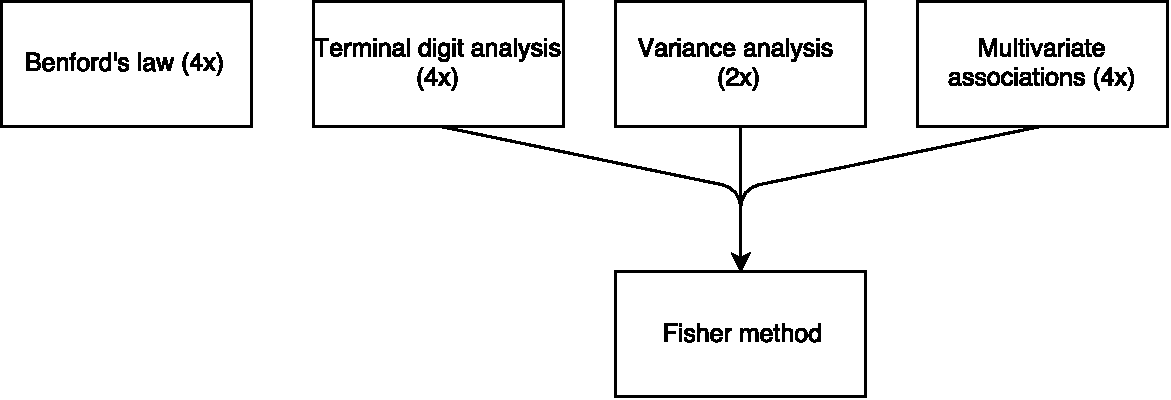
\includegraphics[width=\textwidth,height=\textheight,keepaspectratio]{../figures/study2proc.pdf}
\caption{The applied statistical methods to test for data fabrication in Study 2, depicting those that are combined into an overall test for data fabrication with the Fisher method. Benford’s law is excluded from the overall tests because of an expected lack of utility. Original from \citet{10.3897/rio.2.e8860} under CC-BY.}
\label{study2proc}
\end{center}
\end{figure}

The digit analyses are based on a simple enough premise: test whether the first (i.e., leading) or final (i.e., terminal) digits follow an a priori specified distribution. Benford's law \citep{Benford1938-fl} stipulates that the leading digit follows the distribution of 
\begin{equation}
P(d)=log_{10}(\frac{d+1}{d})
\label{benford}
\end{equation}
where $d$ is the leading digit and $P(d)$ denotes the probability of $d$ (e.g., $P(1)=0.301$). This expected distribution can be tested with a $\chi^2$-test ($df=8$) of the tabular count of leading digits. Similarly, terminal digit analysis \citep{Mosimann1995-av,Mosimann2002-oj} expects that the final digit contains the most measurement error, hence, is uniformly distributed if sufficient digits are available. As a rule of thumb, three digits is sufficient to apply terminal digit analysis \citep{Mosimann1995-av,Mosimann2002-oj}. The observed terminal digit count can be tested against the expected uniform distribution with a $\chi^2$-test as well, although with $df=9$ instead of $df=8$ because a leading digit can never be zero.

We analyzed the variance of the standardized SDs for each condition in each dataset (i.e., two tests per dataset). Whereas in Study 1 the test was conducted on means and standard deviations across cells per study, in Study 2 we conducted the test on means and standard deviations across respondents per condition. The technical aspects of this test remain equivalent to the application in Study 1 (see equations \ref{s2_j} and \ref{simvar}). As such, the only difference is that $N_j$ is no longer the sample size, but the number of Stroop trials presented to the participant.

We analyzed the multivariate associations between the means and standard deviations of the participant-level data in four ways. We computed the observed multivariate associations between the means across conditions (i.e., $r$($M_{congruent}$,$M_{incongruent}$)), the standard deviations across conditions (i.e., $r$($SD_{congruent}$,$SD_{incongruent}$)), and across means and standard deviations within conditions (i.e., $r$($M_{congruent}$,$SD_{congruent}$) and $r$($M_{incongruent}$,$SD_{incongruent}$)). We subsequently compared the observed multivariate correlations from a fabricated dataset with their respective observed multivariate correlations from the genuine data. We computed the probability that the genuine data yielded similar, or more extreme, multivariate correlations (i.e., a $p$-value). Given 21 genuine datasets are available, only 21 $p$-values are possible (i.e., lowest $p$-values possible are 0, 0.048, and 0.095).

We combined the results from the four terminal digit analyses, the two variance analyses, and the four multivariate analyses with the Fisher method. This result was used to determine the top three fabricators, by rank-ordering the $p$-values for each fabricator (higher $p$-value equating to less evidence for fabrication). This omnibus method aggregates evidence from the various methods, making it potentially more sensitive for various fabrication behaviors. We evaluated each of the methods to detect data fabrication using AUROC-curves, using the same procedures as in Study 1.

\section*{Results}

